\documentclass{beamer}
\usepackage{amsmath}
\usepackage{hyperref}
\usepackage{listings}
\usepackage{xcolor}
\hypersetup{colorlinks=true, citecolor=blue, filecolor=blue, linkcolor=blue, urlcolor=blue}
\definecolor{codegreen}{rgb}{0,0.6,0}
\definecolor{codegray}{rgb}{0.5,0.5,0.5}
\definecolor{codepurple}{rgb}{0.58,0,0.82}
\definecolor{backcolour}{rgb}{0.95,0.95,0.92}
 
\lstdefinestyle{mystyle}{
    backgroundcolor=\color{backcolour},   
    commentstyle=\color{codegreen},
    keywordstyle=\color{magenta},
    numberstyle=\tiny\color{codegray},
    stringstyle=\color{codepurple},
    basicstyle=\ttfamily\footnotesize,
    breakatwhitespace=false,         
    breaklines=true,                 
    captionpos=b,                    
    keepspaces=true,                 
    %numbers=left,                    
    numbersep=5pt,                  
    showspaces=false,                
    showstringspaces=false,
    showtabs=false,                  
    tabsize=2
}
 
\lstset{style=mystyle}

\mode<presentation> {

% The Beamer class comes with a number of default slide themes
% which change the colors and layouts of slides. Below this is a list
% of all the themes, uncomment each in turn to see what they look like.

%\usetheme{default}
\usetheme{AnnArbor}
%\usetheme{Antibes}
%\usetheme{Bergen}
%\usetheme{Berkeley}
%\usetheme{Berlin}
%\usetheme{Boadilla}
%\usetheme{CambridgeUS}
%\usetheme{Copenhagen}
%\usetheme{Darmstadt}
%\usetheme{Dresden}
%\usetheme{Frankfurt}
%\usetheme{Goettingen}
%\usetheme{Hannover}
%\usetheme{Ilmenau}
%\usetheme{JuanLesPins}
%\usetheme{Luebeck}
%\usetheme{Madrid}
%\usetheme{Malmoe}
%\usetheme{Marburg}
%\usetheme{Montpellier}
%\usetheme{PaloAlto}
%\usetheme{Pittsburgh}
%\usetheme{Rochester}
%\usetheme{Singapore}
%\usetheme{Szeged}
%\usetheme{Warsaw}

% As well as themes, the Beamer class has a number of color themes
% for any slide theme. Uncomment each of these in turn to see how it
% changes the colors of your current slide theme.

%\usecolortheme{albatross}
%\usecolortheme{beaver}
%\usecolortheme{beetle}
%\usecolortheme{crane}
%\usecolortheme{dolphin}
%\usecolortheme{dove}
%\usecolortheme{fly}
%\usecolortheme{lily}
%\usecolortheme{orchid}
%\usecolortheme{rose}
%\usecolortheme{seagull}
%\usecolortheme{seahorse}
%\usecolortheme{whale}
%\usecolortheme{wolverine}

%\setbeamertemplate{footline} % To remove the footer line in all slides uncomment this line
\setbeamertemplate{footline}[page number] % To replace the footer line in all slides with a simple slide count uncomment this line

\setbeamertemplate{navigation symbols}{} % To remove the navigation symbols from the bottom of all slides uncomment this line
}

\usepackage{graphicx} % Allows including images
\usepackage{booktabs} % Allows the use of \toprule, \midrule and \bottomrule in tables
%\usepackage {tikz}
\usepackage{tkz-graph}
\GraphInit[vstyle = Shade]
\tikzset{
  LabelStyle/.style = { rectangle, rounded corners, draw,
                        minimum width = 2em, fill = yellow!50,
                        text = red, font = \bfseries },
  VertexStyle/.append style = { inner sep=5pt,
                                font = \normalsize\bfseries},
  EdgeStyle/.append style = {->, bend left} }
\usetikzlibrary {positioning}
%\usepackage {xcolor}
\definecolor {processblue}{cmyk}{0.96,0,0,0}
%----------------------------------------------------------------------------------------
%	TITLE PAGE
%----------------------------------------------------------------------------------------

\title[Gradient Descent]{Numerical Optimization 09: Direct Methods} %

\author{Qiang Zhu} % Your name
\institute[University of Nevada Las Vegas] % Your institution as it will appear on the bottom of every slide, may be shorthand to save space
{
University of Nevada Las Vegas\\ % Your institution for the title page
\medskip
}
\date{\today} % Date, can be changed to a custom date

\begin{document}

\begin{frame}
\titlepage % Print the title page as the first slide
\end{frame}

\begin{frame}
\frametitle{Overview} % Table of contents slide, comment this block out to remove it
\tableofcontents % Throughout your presentation, if you choose to use \section{} and \subsection{} commands, these will automatically be printed on this slide as an overview of your presentation
\end{frame}

%----------------------------------------------------------------------------------------
%	PRESENTATION SLIDES
%----------------------------------------------------------------------------------------

%------------------------------------------------

\section{Direct methods without gradient}
\begin{frame}{Direct method}
Direct methods rely solely on the objective function $f$. They are usually called
\begin{itemize}
    \item zero-orther
    \item black box
    \item pattern search
    \item derivative free
\end{itemize}

The most important feature is that they do not rely on derivative information. 
They use other criteria to choose the next search direction to judge if the search is converged.

\end{frame}

\section{Cyclic Coordinate Search}
\begin{frame}{Cyclic Coordinate Search}
This method simply alternate coordinate directions for its line search. The search starts from an initial $\boldsymbol{x}^1$ and optimize the first input.
\begin{columns}

\begin{column}{.6\textwidth}
\begin{equation*}
    \boldsymbol{x}^2 = \underset{x_1}{\arg \min} f(x_1, x_2^1, x_3^1, \cdots, x_n^1) 
\end{equation*}

Then, it moves to the next coordinate,
\begin{equation*}
    \boldsymbol{x}^3 = \underset{x_1}{\arg \min} f(x_1^2, x_2, x_3^2, \cdots, x_n^2) 
\end{equation*}
This process is equivalent to doing a sequence of line searches along the set of $n$ basis vectors.
It is terminated after no significant improvement is made.
\end{column}
\pause
\begin{column}{.4\textwidth}
\begin{figure}
\centering
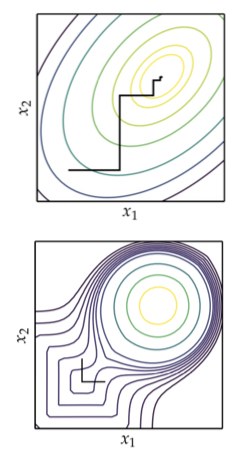
\includegraphics[width=30mm]{Figs/coordinate.jpeg}
\end{figure} 
\end{column}
\end{columns}

\end{frame}

\begin{frame}{Acceleration}
Similar to the momentum method in the gradient descent, the cyclic method can be augmented with an acceleration step to help traverse diagonal valleys. For each full cycle starting with $\boldsymbol{x}^1$ from 1 to $n$, an additional line search is conducted along with 
the direction of $\boldsymbol{x}^{n+1}-\boldsymbol{x}^1$.

\begin{figure}
\centering
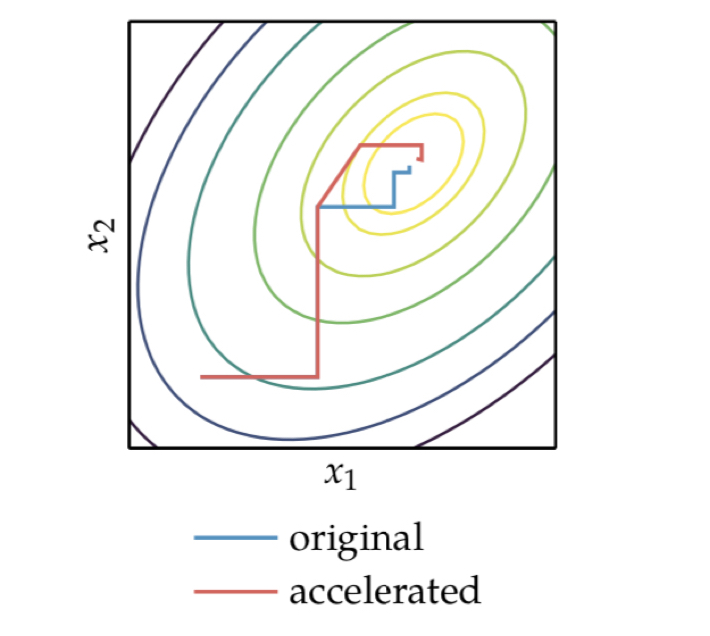
\includegraphics[width=60mm]{Figs/coordinate-improved.jpeg}
\end{figure} 

\end{frame}



\section{Powell's method}
\begin{frame}{Powell's method}
This algorithm maintains a list of search directions $\boldsymbol{u}^1, \cdots, \boldsymbol{u}^n$, which are initially the basis vectors.
Starting at $\boldsymbol{x}^1$, Powell's method conduct a line search for each direction, updating the design point each time,
Then shift each $u$ by one index and drop $u^1$.
The last direction is replaced with the direction of $\boldsymbol{x}^{n+1} - \boldsymbol{x}^1$.


\begin{columns}
\begin{column}{.7\textwidth}
\begin{equation*}
\begin{split}
		\boldsymbol{x}^{i+1} &\leftarrow ~{\textrm{line search}} (f, \boldsymbol{x}^i, \boldsymbol{u}^i) ~{\textrm{for all}} i in 1, \cdots, n\\
		\boldsymbol{u}^{i+1} &\leftarrow \boldsymbol{u}^{i+1} \\~ {\textrm{for all}} i in 1, \cdots, n-1\\
    \boldsymbol{u}^{n} &\leftarrow \boldsymbol{x}^{n+1} - \boldsymbol{x}^n    
\end{split}
\end{equation*}
\end{column}

%\pause
\begin{column}{.3\textwidth}
\begin{figure}
\centering
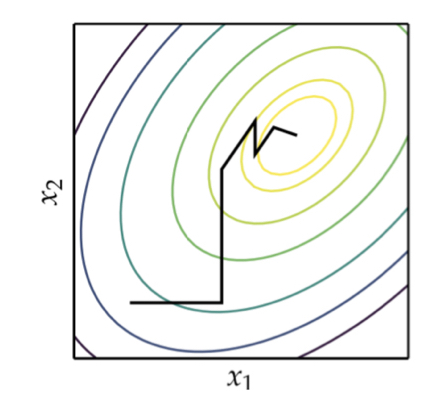
\includegraphics[width=30mm]{Figs/powell.jpeg}
\end{figure} 
\end{column}

\end{columns}

Powell showed that for quadratic functions, after $k$ full iterations the last $k$ direction will be mutually conjugate.
It is recommended to reset every $n$ or $n+1$ iterations.

\end{frame}

\section{Nelder-Mead Simplex Method}
\begin{frame}{Nelder-Mead Simplex Method}

The Nelder-Mead simplex method uses a simplex to traverse the space in search
of a minimum. A simplex is a $n+1$-vertices polyhedron in $n$-dimensional space. 
\begin{columns}
\begin{column}{0.4 \textwidth}
\begin{itemize}
    \item $x_h$, pt of highest $f$, 
    \item $x_s$, pt of 2nd highest $f$, 
    \item $x_l$, pt of lowest $f$, 
    \item $\Bar{x}$, mean pt  excluding $x_h$.
\end{itemize}
\end{column}
\begin{column}{0.6 \textwidth}
\begin{itemize}
    \item Reflection. $x_r = \Bar{x} + (\Bar{x} - x_h)$, 
    \item Expansion. $x_e = \Bar{x} + 2(x_r - \Bar{x})$, 
    \item Contraction. $x_c = \Bar{x} + 0.5(x_h - \Bar{x})$, 
    \item Shrinkage, halving the distance to $x_l$.
\end{itemize}
\end{column}

\end{columns}

\begin{figure}
\centering
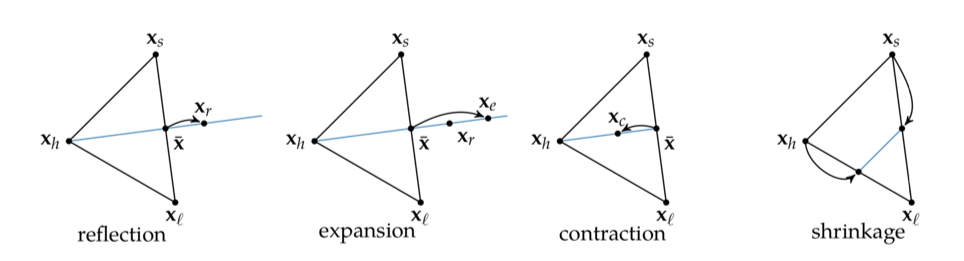
\includegraphics[width=120mm]{Figs/simplex.jpeg}
\end{figure}   
\end{frame}


\begin{frame}{Nelder-Mead Simplex Algorithm}

\begin{figure}
\centering
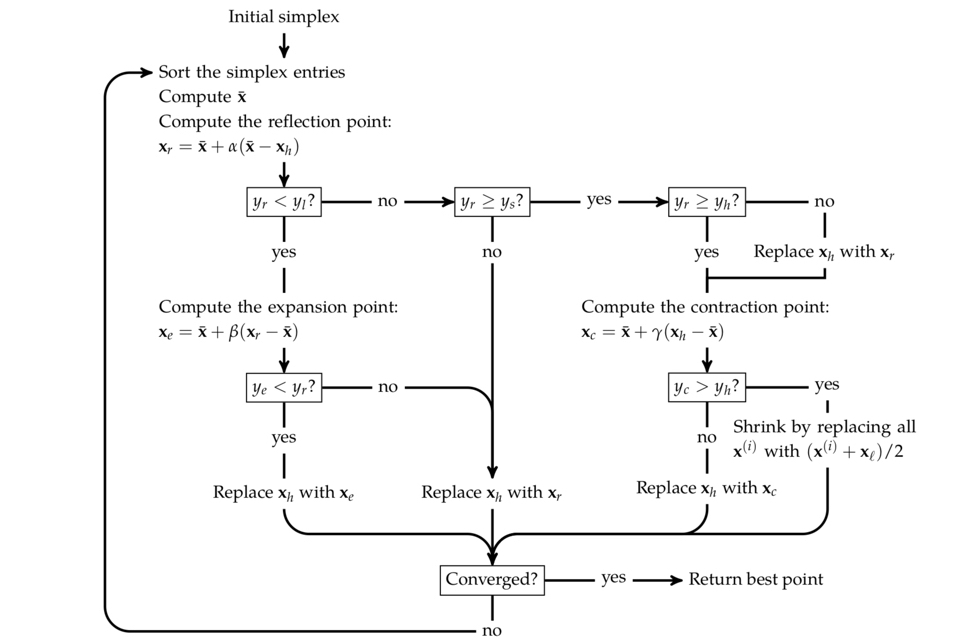
\includegraphics[width=110mm]{Figs/simplex_algo.jpeg}
\end{figure}   
\end{frame}

\begin{frame}{Nelder-Mead Simplex method in practice}

\begin{figure}
\centering
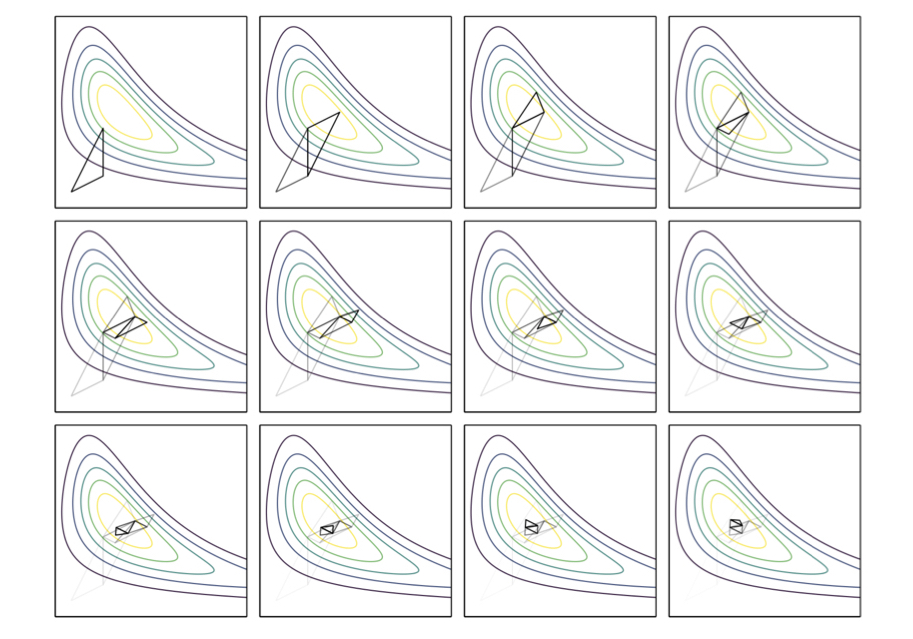
\includegraphics[width=110mm]{Figs/simplex-performance.jpeg}
\end{figure}   
\end{frame}

\section{Summary}
\begin{frame}{Summary}
    \begin{itemize}
        \item Direct methods rely solely on the objective function and do not use derivative information.
        \item Cyclic coordinate search optimizes one coordinate direction at a time.
        \item Powell’s method adapts the set of search directions based on the direction of progress.
        \item The Nelder-Mead simplex method uses a simplex to search the design space, adaptively expanding and contracting the size of the simplex in response to evaluations of the objective function.
    \end{itemize}
\end{frame}
\end{document}

